\documentclass{article}

\usepackage[inner=0.5cm,outer=0.5cm,top=1cm,bottom=0.5cm]{geometry}

\pagestyle{empty}
% This document contains the TikZ-header for all our LaTeX-computations.
% It especially contains all global graphic parameters.

\usepackage{amsmath, amssymb, amsfonts} % Standard Math-stuff

\usepackage{ifthen}

\usepackage{tikz}
\usetikzlibrary{calc}
\usetikzlibrary{positioning}
\usetikzlibrary{shapes}
\usetikzlibrary{patterns}


% Sometimes we want to implement different behaviour for the generated 
% HTML-pictures (for example, shading is not supported in HTML).
% For that we define a macro to check whether we run the code with
% htlatex. The code comes from 
% https://tex.stackexchange.com/questions/93852/what-is-the-correct-way-to-check-for-latex-pdflatex-and-html-in-the-same-latex
\makeatletter
\edef\texforht{TT\noexpand\fi
  \@ifpackageloaded{tex4ht}
    {\noexpand\iftrue}
    {\noexpand\iffalse}}
\makeatother


% Define a text=none option for nodes that ignores the given text, from
% https://tex.stackexchange.com/questions/59354/no-text-none-in-tikz
\makeatletter
\newif\iftikz@node@phantom
\tikzset{
  phantom/.is if=tikz@node@phantom,
  text/.code=%
    \edef\tikz@temp{#1}%
    \ifx\tikz@temp\tikz@nonetext
      \tikz@node@phantomtrue
    \else
      \tikz@node@phantomfalse
      \let\tikz@textcolor\tikz@temp
    \fi
}
\usepackage{etoolbox}
\patchcmd\tikz@fig@continue{\tikz@node@transformations}{%
  \iftikz@node@phantom
    \setbox\pgfnodeparttextbox\hbox{}
  \fi\tikz@node@transformations}{}{}
\makeatother

% Find the angle of a given line (within TikZ)
\newcommand{\tikzAngleOfLine}{\tikz@AngleOfLine}
\def\tikz@AngleOfLine(#1)(#2)#3{%
  \pgfmathanglebetweenpoints{%
    \pgfpointanchor{#1}{center}}{%
    \pgfpointanchor{#2}{center}}
  \pgfmathsetmacro{#3}{\pgfmathresult}%
}

% Now we define the global styles
% The global styles are defined nestedly. You have to give your tikzpicture
% the global options [vertexStyle, edgeStyle, faceStyle] to activate them.
% 
% You can disable labels by using the option nolabels, i.e. 
% vertexStyle=nolabels to deactivate vertex labels.
%
% If you want to have a specific style for your picture, you can also use
% this specific meta-style instead of the general style. For example if you
% want to use double edges in one single picture - no matter the style of
% the rest of the document - you can use edgeDouble instead of edgeStyle.
%
% To set the default style, modify the vertexStyle/.default entry.

% Vertex styles
\tikzset{ 
    vertexNodePlain/.style = {fill=#1, shape=circle, inner sep=0pt, minimum size=2pt, text=none},
    vertexNodePlain/.default=gray,
    vertexPlain/labels/.style = {
        vertexNode/.style={vertexNodePlain=##1},
        vertexLabel/.style={gray}
    },
    vertexPlain/nolabels/.style = {
        vertexNode/.style={vertexNodePlain=##1},
        vertexLabel/.style={text=none}
    },
    vertexPlain/.style = vertexPlain/#1,
    vertexPlain/.default=labels
}
\tikzset{
    vertexNodeNormal/.style = {fill=#1, shape=circle, inner sep=0pt, minimum size=4pt, text=none},
    vertexNodeNormal/.default = blue,
    vertexNormal/labels/.style = {
        vertexNode/.style={vertexNodeNormal=##1},
        vertexLabel/.style={blue}
    },
    vertexNormal/nolabels/.style = {
        vertexNode/.style={vertexNodeNormal=##1},
        vertexLabel/.style={text=none}
    },
    vertexNormal/.style = vertexNormal/#1,
    vertexNormal/.default=labels
}
\tikzset{
    vertexNodeBallShading/pdf/.style = {ball color=#1},
    vertexNodeBallShading/svg/.style = {fill=#1},
    vertexNodeBallShading/.code = {% Conditional shading depending whether we want pdf or svg output
        \if\texforht
            \tikzset{vertexNodeBallShading/svg=#1!90!black}
        \else
            \tikzset{vertexNodeBallShading/pdf=#1}
        \fi
    },
    vertexNodeBall/.style = {shape=circle, vertexNodeBallShading=#1, inner sep=2pt, outer sep=0pt, minimum size=3pt, font=\tiny},
    vertexNodeBall/.default = white,
    vertexBall/labels/.style = {
        vertexNode/.style={vertexNodeBall=##1, text=black},
        vertexLabel/.style={text=none}
    },
    vertexBall/nolabels/.style = {
        vertexNode/.style={vertexNodeBall=##1, text=none},
        vertexLabel/.style={text=none}
    },
    vertexBall/.style = vertexBall/#1,
    vertexBall/.default=labels
}
\tikzset{ 
    vertexStyle/.style={vertexNormal=#1},
    vertexStyle/.default = labels
}


% 1) optional: colour of vertex
% 2) position of the vertex
% 3) relative position of the node
% 4) name of the vertex
\newcommand{\vertexLabelR}[4][]{
    \ifthenelse{ \equal{#1}{} }
        { \node[vertexNode] at (#2) {#4}; }
        { \node[vertexNode=#1] at (#2) {#4}; }
    \node[vertexLabel, #3] at (#2) {#4};
}
% 1) optional: colour of vertex
% 2) position of the vertex
% 3) absolute position of the node
% 4) name of the vertex
\newcommand{\vertexLabelA}[4][]{
    \ifthenelse{ \equal{#1}{} }
        { \node[vertexNode] at (#2) {#4}; }
        { \node[vertexNode=#1] at (#2) {#4}; }
    \node[vertexLabel] at (#3) {#4};
}


% Edge styles
% If you have trouble with the double-lines overlapping, this might (?) help:
% https://tex.stackexchange.com/questions/288159/closing-the-ends-of-double-line-in-tikz
\newcommand{\edgeLabelColor}{blue!20!white}
\tikzset{
    edgeLineNone/.style = {draw=none},
    edgeLineNone/.default=black,
    edgeNone/labels/.style = {
        edge/.style = {edgeLineNone=##1},
        edgeLabel/.style = {fill=\edgeLabelColor,font=\small}
    },
    edgeNone/nolabels/.style = {
        edge/.style = {edgeLineNone=##1},
        edgeLabel/.style = {text=none}
    },
    edgeNone/.style = edgeNone/#1,
    edgeNone/.default = labels
}
\tikzset{
    edgeLinePlain/.style={line join=round, draw=#1},
    edgeLinePlain/.default=black,
    edgePlain/labels/.style = {
        edge/.style={edgeLinePlain=##1},
        edgeLabel/.style={fill=\edgeLabelColor,font=\small}
    },
    edgePlain/nolabels/.style = {
        edge/.style={edgeLinePlain=##1},
        edgeLabel/.style={text=none}
    },
    edgePlain/.style = edgePlain/#1,
    edgePlain/.default = labels
}
\tikzset{
    edgeLineDouble/.style = {very thin, double=#1, double distance=.8pt, line join=round},
    edgeLineDouble/.default=gray!90!white,
    edgeDouble/labels/.style = {
        edge/.style = {edgeLineDouble=##1},
        edgeLabel/.style = {fill=\edgeLabelColor,font=\small}
    },
    edgeDouble/nolabels/.style = {
        edge/.style = {edgeLineDouble=##1},
        edgeLabel/.style = {text=none}
    },
    edgeDouble/.style = edgeDouble/#1,
    edgeDouble/.default = labels
}
\tikzset{
    edgeStyle/.style = {edgePlain=#1},
    edgeStyle/.default = labels
}

% Face styles
% Here we have an exception - the style face is always defined.
% 
\newcommand{\faceColorY}{yellow!60!white}   % yellow
\newcommand{\faceColorB}{blue!60!white}     % blue
\newcommand{\faceColorC}{cyan!60}           % cyan
\newcommand{\faceColorR}{red!60!white}      % red
\newcommand{\faceColorG}{green!60!white}    % green
\newcommand{\faceColorO}{orange!50!yellow!70!white} % orange

% define default face colour (and default swap colour)
\newcommand{\faceColor}{\faceColorY}
\newcommand{\faceColorSwap}{\faceColorC}

% define secondary default colours (to use in a single section)
\newcommand{\faceColorFirst}{green!40!white}
\newcommand{\faceColorSecond}{gray!15!white}
\newcommand{\faceColorThird}{red!17!white}
\newcommand{\faceColorFourth}{olive!20!white}

\tikzset{
    face/.style = {fill=#1},
    face/.default = \faceColor,
    faceY/.style = {face=\faceColorY},
    faceB/.style = {face=\faceColorB},
    faceC/.style = {face=\faceColorC},
    faceR/.style = {face=\faceColorR},
    faceG/.style = {face=\faceColorG},
    faceO/.style = {face=\faceColorO}
}
\tikzset{
    faceStyle/labels/.style = {
        faceLabel/.style = {}
    },
    faceStyle/nolabels/.style = {
        faceLabel/.style = {text=none}
    },
    faceStyle/.style = faceStyle/#1,
    faceStyle/.default = labels
}
\tikzset{ face/.style={fill=#1} }
\tikzset{ faceSwap/.code=
    \ifdefined\swapColors
        \tikzset{face=\faceColorSwap}
    \else
        \tikzset{face=\faceColor}
    \fi
}



\usepackage{hyperref}


\begin{document}



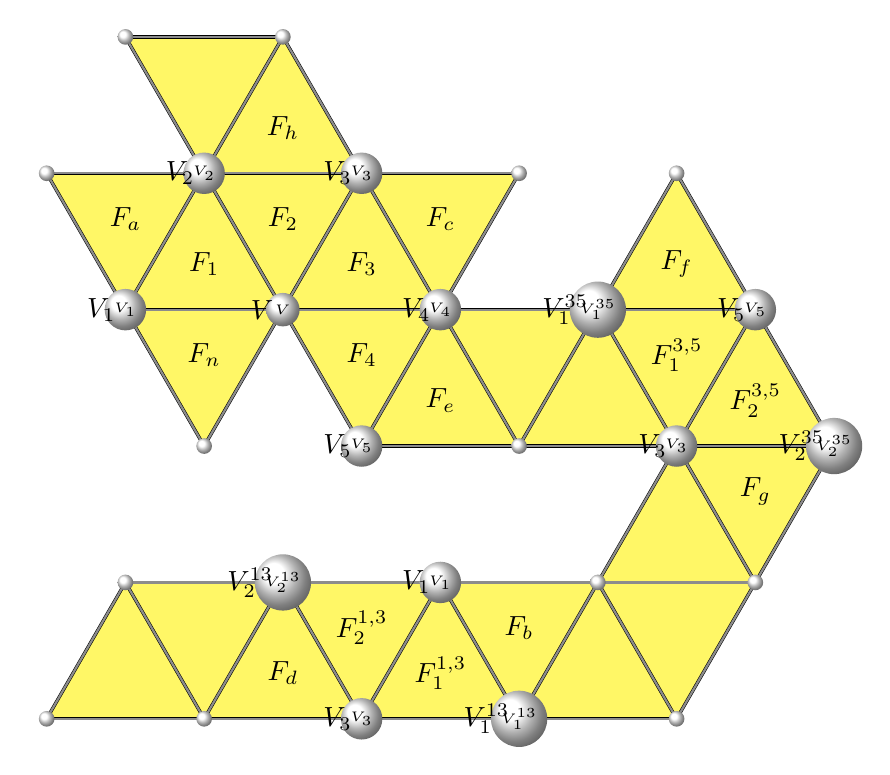
\begin{tikzpicture}[vertexBall, edgeDouble, faceStyle, scale=2]

% Define the coordinates of the vertices
\coordinate (V1_1) at (0.4999999999999999, 0.8660254037844386);
\coordinate (V2_1) at (0, 0);
\coordinate (V3_1) at (2, -1.732050807568877);
\coordinate (V4_1) at (3, -1.732050807568876);
\coordinate (V5_1) at (3.5, -0.8660254037844379);
\coordinate (V5_2) at (3.5, -2.598076211353314);
\coordinate (V6_1) at (1.500000000000001, -2.598076211353316);
\coordinate (V7_1) at (2.000000000000002, -3.464101615137753);
\coordinate (V7_2) at (0.5000000000000018, -2.598076211353316);
\coordinate (V8_1) at (3, 0);
\coordinate (V8_2) at (3.000000000000001, -3.464101615137752);
\coordinate (V9_1) at (0, -1.732050807568879);
\coordinate (V10_1) at (2, 0);
\coordinate (V11_1) at (-1, 1.732050807568877);
\coordinate (V11_2) at (-1, -1.732050807568881);
\coordinate (V12_1) at (1.5, -0.8660254037844385);
\coordinate (V12_2) at (-1.5, 0.8660254037844379);
\coordinate (V13_1) at (1.5, 0.8660254037844387);
\coordinate (V13_2) at (0, 1.732050807568877);
\coordinate (V13_3) at (-1.499999999999998, -2.598076211353321);
\coordinate (V14_1) at (0.5, -0.8660254037844386);
\coordinate (V14_2) at (-0.9999999999999996, 0);
\coordinate (V15_1) at (1, 0);
\coordinate (V15_2) at (2.500000000000001, -2.598076211353315);
\coordinate (V15_3) at (2.5, 0.8660254037844384);
\coordinate (V15_4) at (-0.4999999999999982, -2.598076211353319);
\coordinate (V16_1) at (-0.5, 0.8660254037844384);
\coordinate (V16_2) at (2.5, -0.8660254037844383);
\coordinate (V16_3) at (1.000000000000001, -1.732050807568878);
\coordinate (V16_4) at (-0.5000000000000021, -0.866025403784441);


% Fill in the faces
\fill[face]  (V2_1) -- (V16_4) -- (V14_2) -- cycle;
\node[faceLabel] at (barycentric cs:V2_1=1,V16_4=1,V14_2=1) {$F_n$};
\fill[face]  (V15_1) -- (V1_1) -- (V2_1) -- cycle;
\node[faceLabel] at (barycentric cs:V15_1=1,V1_1=1,V2_1=1) {$F_3$};
\fill[face]  (V16_2) -- (V3_1) -- (V4_1) -- cycle;
%\node[faceLabel] at (barycentric cs:V16_2=1,V3_1=1,V4_1=1) {$2$};
\fill[face]  (V1_1) -- (V16_1) -- (V2_1) -- cycle;
\node[faceLabel] at (barycentric cs:V1_1=1,V16_1=1,V2_1=1) {$F_2$};
\fill[face]  (V16_1) -- (V14_2) -- (V2_1) -- cycle;
\node[faceLabel] at (barycentric cs:V16_1=1,V14_2=1,V2_1=1) {$F_1$};
\fill[face]  (V1_1) -- (V13_2) -- (V16_1) -- cycle;
\node[faceLabel] at (barycentric cs:V1_1=1,V13_2=1,V16_1=1) {$F_h$};
\fill[face]  (V16_1) -- (V12_2) -- (V14_2) -- cycle;
\node[faceLabel] at (barycentric cs:V16_1=1,V12_2=1,V14_2=1) {$F_a$};
\fill[face]  (V13_2) -- (V11_1) -- (V16_1) -- cycle;
\node[faceLabel] at (barycentric cs:V13_2=1,V11_1=1,V16_1=1) {$ $};
\fill[face]  (V12_1) -- (V16_2) -- (V10_1) -- cycle;
%\node[faceLabel] at (barycentric cs:V12_1=1,V16_2=1,V10_1=1) {$8$};
%\fill[face]  (V9_1) -- (V16_4) -- (V11_2) -- cycle;
%\node[faceLabel] at (barycentric cs:V9_1=1,V16_4=1,V11_2=1) {$9$};
\fill[face]  (V16_2) -- (V8_1) -- (V10_1) -- cycle;
\node[faceLabel] at (barycentric cs:V16_2=1,V8_1=1,V10_1=1) {$F_1^{3,5}$};
\fill[face]  (V16_3) -- (V9_1) -- (V7_2) -- cycle;
\node[faceLabel] at (barycentric cs:V16_3=1,V9_1=1,V7_2=1) {$F_2^{1,3}$};
\fill[face]  (V16_2) -- (V5_1) -- (V8_1) -- cycle;
\node[faceLabel] at (barycentric cs:V16_2=1,V5_1=1,V8_1=1) {$F_2^{3,5}$};
\fill[face]  (V16_3) -- (V7_2) -- (V6_1) -- cycle;
\node[faceLabel] at (barycentric cs:V16_3=1,V7_2=1,V6_1=1) {$F_1^{1,3}$};
\fill[face]  (V16_2) -- (V4_1) -- (V5_1) -- cycle;
\node[faceLabel] at (barycentric cs:V16_2=1,V4_1=1,V5_1=1) {$F_g$};
\fill[face]  (V3_1) -- (V16_3) -- (V6_1) -- cycle;
\node[faceLabel] at (barycentric cs:V3_1=1,V16_3=1,V6_1=1) {$F_b$};
\fill[face]  (V14_1) -- (V12_1) -- (V15_1) -- cycle;
\node[faceLabel] at (barycentric cs:V14_1=1,V12_1=1,V15_1=1) {$F_e$};
\fill[face]  (V11_2) -- (V13_3) -- (V15_4) -- cycle;
%\node[faceLabel] at (barycentric cs:V11_2=1,V13_3=1,V15_4=1) {$17$};
\fill[face]  (V3_1) -- (V15_2) -- (V4_1) -- cycle;
%\node[faceLabel] at (barycentric cs:V3_1=1,V15_2=1,V4_1=1) {$18$};
%\fill[face]  (V15_2) -- (V5_2) -- (V4_1) -- cycle;
%\node[faceLabel] at (barycentric cs:V15_2=1,V5_2=1,V4_1=1) {$19$};
\fill[face]  (V3_1) -- (V6_1) -- (V15_2) -- cycle;
%\node[faceLabel] at (barycentric cs:V3_1=1,V6_1=1,V15_2=1) {$20$};
%\fill[face]  (V15_2) -- (V8_2) -- (V5_2) -- cycle;
%\node[faceLabel] at (barycentric cs:V15_2=1,V8_2=1,V5_2=1) {$21$};
%\fill[face]  (V6_1) -- (V7_1) -- (V15_2) -- cycle;
%\node[faceLabel] at (barycentric cs:V6_1=1,V7_1=1,V15_2=1) {$22$};
\fill[face]  (V8_1) -- (V15_3) -- (V10_1) -- cycle;
\node[faceLabel] at (barycentric cs:V8_1=1,V15_3=1,V10_1=1) {$F_f$};
\fill[face]  (V9_1) -- (V15_4) -- (V7_2) -- cycle;
\node[faceLabel] at (barycentric cs:V9_1=1,V15_4=1,V7_2=1) {$F_d$};
\fill[face]  (V12_1) -- (V10_1) -- (V15_1) -- cycle;
%\node[faceLabel] at (barycentric cs:V12_1=1,V10_1=1,V15_1=1) {$25$};
\fill[face]  (V9_1) -- (V11_2) -- (V15_4) -- cycle;
%\node[faceLabel] at (barycentric cs:V9_1=1,V11_2=1,V15_4=1) {$26$};
\fill[face]  (V2_1) -- (V14_1) -- (V15_1) -- cycle;
\node[faceLabel] at (barycentric cs:V2_1=1,V14_1=1,V15_1=1) {$F_4$};
\fill[face]  (V15_1) -- (V13_1) -- (V1_1) -- cycle;
\node[faceLabel] at (barycentric cs:V15_1=1,V13_1=1,V1_1=1) {$F_c$};


% Draw the edges
\draw[edge] (V14_2) --  (V16_4);
\draw[edge] (V2_1) --  (V16_4);
\draw[edge] (V15_1) --  (V2_1);
\draw[edge] (V15_1) --  (V2_1);
\draw[edge] (V1_1) --  (V15_1);
\draw[edge] (V4_1) --  (V16_2);
\draw[edge] (V3_1) -- (V16_2);
\draw[edge] (V16_3) --  (V3_1);
\draw[edge] (V2_1) --  (V16_1);
\draw[edge] (V16_1) --  (V1_1);
\draw[edge] (V14_2) --  (V16_1);
\draw[edge] (V16_1) -- (V13_2);
\draw[edge] (V12_2) -- (V16_1);
\draw[edge] (V16_2) -- (V12_1);
\draw[edge] (V16_1) -- (V11_1);
%\draw[edge] (V11_2) -- (V16_4);
\draw[edge] (V10_1) -- (V16_2);
\draw[edge] (V9_1) -- (V16_3);
%\draw[edge] (V16_4) -- (V9_1);
\draw[edge] (V8_1) -- (V16_2);
\draw[edge] (V7_2) -- (V16_3);
\draw[edge] (V5_1) -- (V16_2);
\draw[edge] (V6_1) -- (V16_3);
\draw[edge] (V4_1) -- (V15_2);
\draw[edge] (V15_2) -- (V3_1);
%\draw[edge] (V5_2) -- (V15_2);
\draw[edge] (V15_2) -- (V6_1);
%\draw[edge] (V8_2) -- (V15_2);
\draw[edge] (V15_3) -- (V8_1);
%\draw[edge] (V15_2) -- (V7_1);
\draw[edge] (V7_2) -- (V15_4);
\draw[edge] (V15_1) -- (V10_1);
\draw[edge] (V10_1) -- (V15_3);
\draw[edge] (V15_4) -- (V9_1);
\draw[edge] (V15_1) -- (V12_1);
\draw[edge] (V15_4) -- (V11_2);
\draw[edge] (V15_1) -- (V14_1);
\draw[edge] (V13_1) -- (V15_1);
\draw[edge] (V15_4) -- (V13_3);
\draw[edge] (V2_1) -- (V1_1);
\draw[edge] (V4_1) -- (V3_1);
\draw[edge] (V5_1) -- (V4_1);
%\draw[edge] (V4_1) -- (V5_2);
\draw[edge] (V6_1) -- (V3_1);
\draw[edge] (V8_1) -- (V5_1);
%\draw[edge] (V5_2) -- (V8_2);
%\draw[edge] (V7_1) -- (V6_1);
\draw[edge] (V6_1) -- (V7_2);
\draw[edge] (V10_1) --  (V8_1);
\draw[edge] (V7_2) --  (V9_1);
\draw[edge] (V10_1) --  (V12_1);
\draw[edge] (V11_2) --  (V9_1);
\draw[edge] (V12_1) --  (V14_1);
\draw[edge] (V14_2) --  (V12_2);
\draw[edge] (V11_1) --  (V13_2);
\draw[edge] (V13_3) --  (V11_2);
\draw[edge] (V14_1) --  (V2_1);
\draw[edge] (V2_1) --  (V14_2);
\draw[edge] (V1_1) --  (V13_1);
\draw[edge] (V13_2) -- (V1_1);


% Draw the vertices
\vertexLabelR{V1_1}{left}{$V_3$}
\vertexLabelR{V2_1}{left}{$V$}
\vertexLabelR{V3_1}{left}{$ $}
\vertexLabelR{V4_1}{left}{$ $}
\vertexLabelR{V5_1}{left}{$V_2^{35}$}
%\vertexLabelR{V5_2}{left}{$5$}
\vertexLabelR{V6_1}{left}{$V_1^{13}$}
%\vertexLabelR{V7_1}{left}{$7$}
\vertexLabelR{V7_2}{left}{$V_3$}
\vertexLabelR{V8_1}{left}{$V_5$}
%\vertexLabelR{V8_2}{left}{$ $}
\vertexLabelR{V9_1}{left}{$V_2^{13}$}
\vertexLabelR{V10_1}{left}{$V_1^{35}$}
\vertexLabelR{V11_1}{left}{$ $}
\vertexLabelR{V11_2}{left}{$ $}
\vertexLabelR{V12_1}{left}{$ $}
\vertexLabelR{V12_2}{left}{$ $}
\vertexLabelR{V13_1}{left}{$ $}
\vertexLabelR{V13_2}{left}{$ $}
\vertexLabelR{V13_3}{left}{$ $}
\vertexLabelR{V14_1}{left}{$V_5$}
\vertexLabelR{V14_2}{left}{$V_1$}
\vertexLabelR{V15_1}{left}{$V_4$}
\vertexLabelR{V15_2}{left}{$ $}
\vertexLabelR{V15_3}{left}{$ $}
\vertexLabelR{V15_4}{left}{$ $}
\vertexLabelR{V16_1}{left}{$V_2$}
\vertexLabelR{V16_2}{left}{$V_3$}
\vertexLabelR{V16_3}{left}{$V_1$}
\vertexLabelR{V16_4}{left}{$ $}

\end{tikzpicture}
\end{document}
